\subsection{Distributed File Sharing}
\label{subsec:design-p2p}

\subsubsection*{Hash Tree}
\label{subsubsec:hash-tree}

The Hash Tree of a given directory is used to represent its structure as well as the contents of its files. Each file is represented by an ordered list of SHA-256 hashes that match a fixed-size shard of data. This allows users to easily identify and verify game data.

\begin{figure}[ht]
  \centering
  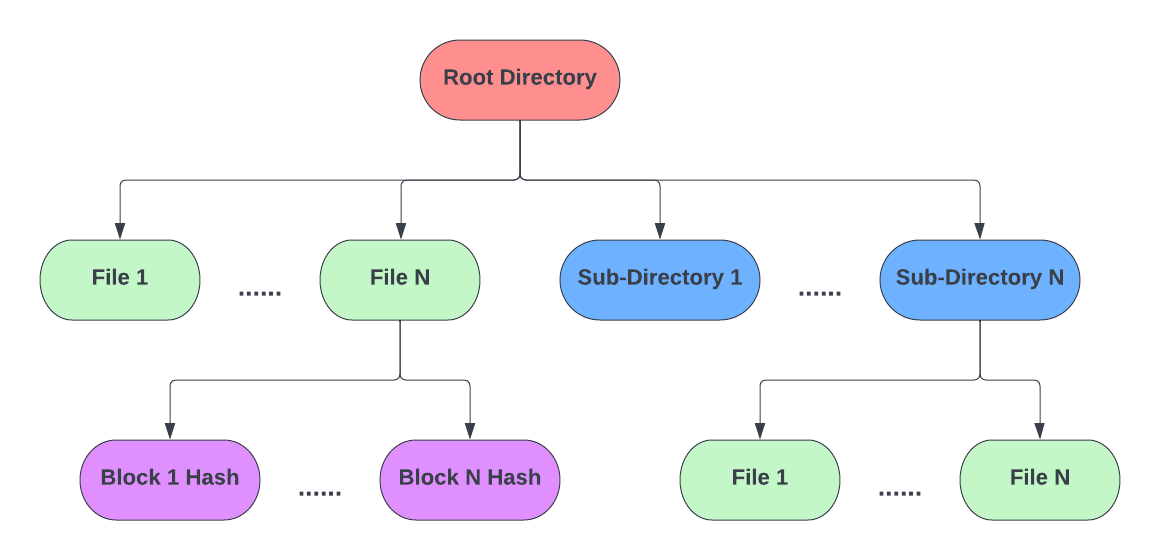
\includegraphics[width=.85\textwidth]{assets/images/diagrams/block-body.png}
  \caption{The structure of a Hash Tree}
  \label{fig:hash-storage}
\end{figure}

\subsubsection*{Uploading Content}
\label{subsubsec:upload-content}

For a developer to upload their game \reqref{F-M5} they must provide the required metadata outlined in Section~\ref{subsubsec:eth-data} as well as the location of the game in storage. A Hash Tree is then generated and all data is sent to its corresponding platform. The game is added to the uploader's library and can now be downloaded from other users who have purchased it.

\subsubsection*{Downloading Content}

Like mentioned in Section~\ref{subsec:design-data}, it is impractical to store the game's data on the blockchain or IPFS. Instead we will consider ideas from decentralised file-sharing networks, like discussed in Sections~\ref{sec:lit-p2p} \&~\ref{sec:bittorrent}.
\x
Games are content addressable using their root hash which will allow a user to discover peers who share the same games as them and request blocks of data from them \reqref{F-C3}. When a peer seeking data forms a connection with another peer they will:

\begin{enumerate}
  \item Perform a handshake to determine each other's Ethereum address and public key.
  \item The seeder will verify that the downloader owns the game by checking the \textit{purchased} mapping on the Smart Contract.
  \item The downloader will send requests for individual blocks to the seeder \reqref{F-M2}.
  \item Upon receiving a block, the downloader will verify the contents using the block's hash \reqref{F-M7}.
  \item Repeat Steps 3--4 for an arbitrary number of blocks.
  \item The seeder may request a signed receipt that details the blocks they uploaded.
\end{enumerate}

\subsubsection*{Updating Content}\label{subsubsec:updating}

To satisfy \reqref{F-M4}, developers will perform the same steps outlined in Section~\ref{subsubsec:upload-content} but must also provide the root hash of the most previous version of the game. Any users who have purchased the previous version, will be added to the list of users who have purchased the new version. Additionally, this will include the restriction that only the original uploader can upload an update for their game \reqref{NF-S2}.
\x
Each version is considered as its own game and will require users to download the updated version separately. Whilst this isn't reflective of how updates are typically managed, this will be acceptable for the scope of this project and any changes will be considered as a future extension to this project.

\subsubsection*{Downloadable Content}

Downloadable Content DLC represent optional additions for games that users will buy separately. DLCs will act similarly to how updates are treated. Each DLC will need:

\begin{enumerate}
  \item \textbf{Dependency} The root hash of the oldest version of the game this DLC supports.
  \item \textbf{Previous Version} (Optional) The root hash of the previous version of the DLC.
\end{enumerate}

\subsubsection*{Proving Contribution}

As a user downloads blocks of data, they will keep track of which users have sent them which blocks. A peer may then request their contributions in the form of a signed message that can be sent the developer \reqref{F-S1} in return for some kind of reward. The contents of the reward isn't specified for this project but could include in-game items, digital assets or Ether.